\documentclass[tikz,border=10pt]{standalone}
\usepackage[T1]{fontenc}
\usepackage{lmodern}
\usetikzlibrary{arrows.meta,positioning}
\definecolor{ink}{HTML}{183444}
\definecolor{blue}{HTML}{1B6780}
\definecolor{amber}{HTML}{AD601A}
\begin{document}
\hyphenpenalty=10000\exhyphenpenalty=10000
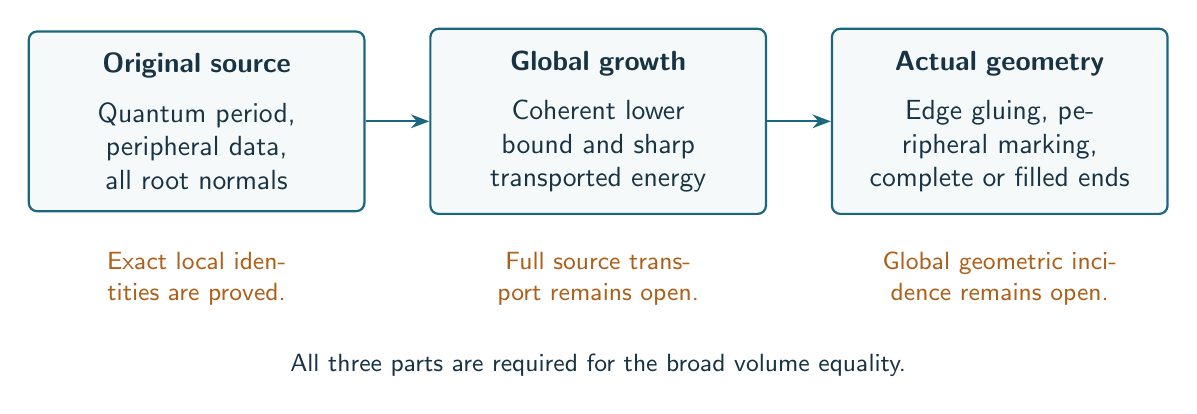
\begin{tikzpicture}[font=\sffamily,text=ink,>=Stealth,
 box/.style={draw=blue,thick,rounded corners=3pt,fill=blue!4,text width=3.7cm,minimum height=2.1cm,align=center,inner sep=8pt},
 gap/.style={text width=4cm,align=center,font=\sffamily\small,text=amber}]
 \node[box] (s) at (0,0) {\textbf{Original source}\\[6pt]Quantum period, peripheral data, all root normals};
 \node[box] (e) at (5.1,0) {\textbf{Global growth}\\[6pt]Coherent lower bound and sharp transported energy};
 \node[box] (g) at (10.2,0) {\textbf{Actual geometry}\\[6pt]Edge gluing, peripheral marking, complete or filled ends};
 \draw[->,thick,blue] (s)--(e);
 \draw[->,thick,blue] (e)--(g);
 \node[gap] at (0,-2) {Exact local identities are proved.};
 \node[gap] at (5.1,-2) {Full source transport remains open.};
 \node[gap] at (10.2,-2) {Global geometric incidence remains open.};
 \node[font=\sffamily\small,text=ink] at (5.1,-3.1) {All three parts are required for the broad volume equality.};
\end{tikzpicture}
\end{document}
